\begin{center}\small{
Beware the contents of this tale,\\
for in them lies a man so frail\\
that he does think death is release\\
and tries to make his own life cease.}
\end{center}
Drip.

Silence pervaded the very pores of the city, as the winds did not dare to make even the slightest of squeaks, simply floating imperceptibly over the irregular skylines of modernity. Between the dark crevices of endless buildings, lonesome streetlights flickered, humming only occasionally with surges of electricity. They illuminated potholes, straits of tarmac, and orange cones which waited expectantly for the rabid destruction of the lands they guarded.  The lights unveiled dumps of plastic bottles, cans and dried chewing gum within the borders of the city, as they danced together in their unlikely choreographies.

Drip.

Through the city ran a meandering lifeline. A source of hope for many, and the promise of death for others. A once glassy river flowed playfully through it all. The river breathed deeply, rising and falling, ebbing and flowing, being the only constant in a city that changed every day. The lovelorn embankments gave way to their desire to accompany the river as they crumbled slowly, gently, joining its seemingly endless flow in the hopes of finding an adventure.

Drip.

The twinkling stars extinguished in the river’s reflection as her waters tumble over themselves, till each star was naught but a ripple. And yet a single celestial body could not be dimmed despite the river’s valiant efforts to submerge it. The half-moon gleamed defiantly in her waters, gleefully sweeping over the river, and latching onto everything that light may touch. The moon’s light shone through gaps between monuments, from reflections off billboards, and directly onto the river itself. The moon sought out every seemingly unimportant fracture in her nightly quest and always waited patiently for when the sun grew weary.

Drip.

Moonlight swept over the black hair of a man, whose face was marked with glimmering streaks. His lengthy black coat was dishevelled and his dress shoes were caked in mud. A heavy rock scratched his soft hands. A glib drop swelled in his brown eyes and trickled down his face, collecting on his still hairless chin.

Drip.                                

The tear disappeared into the river, melting into its lively stream. His lips quivered and his body shook as he pulled on the thick rope wrapped around the rock. It tugged on his leg, but remained firm, establishing itself like another limb. He exhaled meekly, colouring the air white. He hugged the rock close like a child clinging to a teddy bear and climbed onto the ledge of the bridge. Goosebumps rose over his flesh, and the hairs on the back of his neck stood on end, as the hollowness began spreading through his abdomen. The cocoon-like layers of clothing did nothing to warm his icy limbs. He did not need to put his hand into his pocket to feel the weight of the innocuous papers that made him long for the bottom of the ocean. When there is no ocean, rivers must do. 

\emph{Just one step. It will all be over. Just… one…single... step. Then I can be rid of all the pain and troubles and burdens…}

A cat weaved through his legs and meowed beside him. Startled, he lost his footing and fell forward. The clocks sped ahead, the years turning to days, the days to hours, the hours to seconds, and the seconds to mere instants, and yet he felt everything in excruciating slowness.

He watched as the rock fell down ahead of him, his body following it slowly as he dove in feet first, breaking the surface of the icy stream. The water gleamed white as it jumped up in response, hailing down once his entire body was submerged.

\emph{No!} The thought rung out in his mind, clear and crisp as a fresh day. He began flapping his arms desperately and kicked furiously as he struggled to fight the rock which weighed him down.

\emph{No, no, I want to live!} The thoughts attacked his skull as realisation dawned on him. This world is no fairy tale. There are no swift and merciful endings. It is a dire and ugly place filled with much that is unbearable, but some things cannot be abandoned. \emph{I want life!}

He tugged on the rock, trying to pick it up, but somehow a thick chain of seaweed had wrapped itself around the rock, anchoring him into place. He struggled and pulled, scratching like a ferocious beast at the seaweed, not noticing the pitch-black eyes in the distance.

A series of large bubbles escaped his lips. 

Everything grew blurry... darker... unfocused…

\emph{No, please…} he thought once more, hand outstretched in the direction of the water surface where the moon shone brightly. \emph{No…}

His body began relenting, hope and life draining from him, as he closed his hand around the moon in one last plea.

\emph{What…?}

Instead of grasping water, a half-moon shaped blade cut into his palm, drawing blood.

\emph{How…?}

\emph{Don’t ask questions, Endymion. Save yourself}, a voice breathed intimately as if it whispered from beside him.

With his last shred of his strength, he brought the blade to the rope and began slashing at it, gritting his teeth together. It frayed with each uncoordinated stroke, as the stream kept fighting against his hand. Dark, rusty blood fled from the blade as the rope relented at last.

All he saw was water. Dark, murky, twisting, unyielding water which held him down despite every stroke of his legs. It pressed down, pushing him along like a ragdoll. Tossing him over and over, until he couldn’t tell up from down, left from right, and lost the blade in the vastness of the river. He stared dazedly into the distance where incorporeal souls lamented; pity and sadness emanating from them. Their translucent selves floated along the riverbed, wandering downstream. They reached up for him and turned their faceless forms towards him.

\emph{The light, Endymion. The light}, whispered the same strange voice. Blinking drowsily, and unable to focus, he saw the moonlight filter through the waves. But it was too late.

Everything went dark. 

He didn’t hear the waves. He didn’t hear his frantic heartbeat. He didn’t hear the blood-curdling scream that shattered the night. He didn’t feel the cool, inhuman fingers which wrapped around his wrist. He didn’t feel the slap of fresh air as he broke to the surface of the river, to a land that looked nothing like the one he had left behind.

His body resurfaced in the midst of a barren world, with death cradling both sides of the embankment, in the form of rotting trees and parched lands. The skies were crimson blood, and in the distance stood a ferry, made of old well-worn wood, whose polish flaked from its sharp body. Upon the ferry stood a lonesome ferryman holding an oar upon his shoulders, watching intently. His wrinkled face twisted in wry amusement, as he watched with interest.

In Endymion’s unconscious state, he did not feel a dozen wraiths wrap themselves around his legs, trying to drag him down. Nor did he feel the soft glow, from the inhuman white hand entering into his forehead, nor feel it spreading into his core and sliding over his skin. The light wrapped itself around his body and illuminated him from within until the wraiths let go, hissing in agony.

\emph{Stop that, Selene! He entered the realm of hate, and that makes him my rightful acquisition}, an angry voice announced, surfacing upstream. Liquids dripped from the creature’s body, spilling like ink from the dark-red dulse which hung from her head. On her head was a crown of young starfish, entangled with several strands of seaweed, crowning her fae-body. A sea lamprey slung tightly around the waist of her knee-length zebra mussel dress, reflecting in the black pool that the river had become. The gills on her upper arm flared briefly, threateningly displaying a luminous green layer beneath her scale shoulder-pads. She glowered, her jet black eyes focused on the glowing, seemingly-immaterial, figure who carried Endymion in her arms, cradling the unconscious form protectively.

\emph{He fell by accident, Styx. He was not yours to drown.}

\emph{I can do what I want to those who attempt to end their miserable existences.}

\emph{And yet you insisted on trying to kill him even when he had a change of heart. You know as well as I do that this is not his place.}

Styx’s gills flared again. \emph{You have no right to judge my decisions.} With a flick of her wrist, a wall of water rose from where she stood, piling onto itself until there was a plunging wave that should have dried out any other river but the Styx. With one fell swoop of Selene’s wrist, the wave split apart in the middle and crashed down on either side of Endymion.

\emph{Do not try to challenge me, Styx. I control the seas, the tides and the winds of this world. You are nothing but a little pawn in Hades’ game.}

\emph{I am no such thing}, Styx growled, black eyes wide with fury. Her teeth gleamed as she propelled towards them, breaking easily through the walls of water that sprung up with each of Selene’s hand gestures. Styx’ tail oscillated frantically, as she closed the distance between them.

Sucking in a sharp breath, Selene clutched Endymion and covered his eyes with her hand.

A bright light burst forth from her body, and pushed Styx back. From below the water surface, the faceless wraiths briefly regained the lights of their eyes and swam to the surface. They gazed upon the unnatural brightness, tilting their heads in awe before the light dimmed once again. With that, the ones closest to Styx grabbed onto her as they reverted to their previous state, and pulled her into the depths with them.

From the distance, a low, boisterous laugh filled the empty landscape.

“Charon?”

“I must admit this has been a most entertaining night, Selene. Styx shall be furious once she breaks free from the damned.” He beamed at her, as he stood in his ferry, leaning against the oar casually, his blue-green eyes glittering in her remnant glow.

“You do not think she is in the right?” Selene asked, levitating towards him, while never letting go of the prized mortal.

“We both know that Styx's claim is a true one. The life was forfeit, whether his appearance on my river was by choice or not. But as you have both meddled in his fate this night… I shan’t force you to give this one to Hades just yet.” He smirked at the man, and touched his forehead briefly, creating a small flame which entered into his body. “And as I am now feeling quite genial, I shall even grant him safe passage without payment when the time comes for his true departure.”

“Thank you,” she breathed a sigh of relief.

``There is no need to thank me, young one. There is still much to be learnt by you and the mortal."

“This mortal is different," she insisted. ``I can feel this one can achieve much among his kind. I have watched them for so long from the skies, and I am certain that greatness slumbers in this one’s bosom.”

“I am sure you are right,” chortled Charon, his shoulder-length grey hair dancing as a light breeze drifted through the wastelands of the underworld. “Forget not, you ought to take him away before Styx resurfaces,” he grinned.

Selene nodded, and her broad lips spread into a smile as they faded away once more.

---

Endymion jolted awake on a park bench, gasping for air. The park was quiet, with only a few birds chirping playfully as they flew around to feed their young. The pastel sky glowed dimly as Endymion sat upright and covered his mouth to yawn.

“It is a lovely morning, is it not?”

Startled, he looked up to see a white-haired, young woman sitting on the edge of the park bench, her face hidden away behind her broad-brimmed, black sunhat.

“I-I guess…”

“I thrive for the nights, but there is something comforting about the knowledge that even the longest nights- and days too- come to an end. It is nearly... cathartic, Endymion.”

“I’m sorry, do I know you from somewhere?” He furrowed his brow and pulled his legs closer to his chest to give her more space on the bench.

“Everyone does,” she laughed brightly, as she stood up, her plain chiffon dress seemingly floating in the soft breeze. “Next time, spend your nights dreaming and your days living them,” she beamed, and her silver eyes sparkled as she beheld him.

A fresh beam of sunlight filtered through the leaves and blinded him. By the time he had raised his hands to block the light, the woman was gone.

He frowned deeply, and looked around for any sign of her, rubbing his eyes and blinking a couple times. He rose from the bench and walked into the meadow, searching for the woman, until a soft luminosity caught his eye. Up above in the sky, the half-moon shone faintly, fading away as the sun took over the heavens.

Before he knew it, he had slung his coat over his shoulder, basking in the early morning light, and walked through the park humming Claire de Lune.
%
%\begin{figure}[h!]
%\centering
%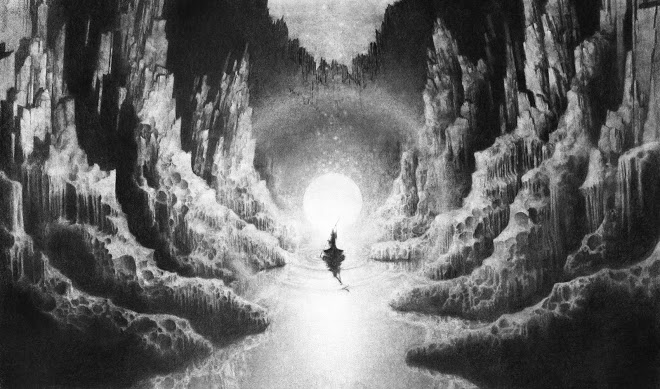
\includegraphics[width=0.6\textwidth]{./pictures/styx}
%\end{figure}
